\section{Theoretical background and literature review}
\label{section:2}

\subsection{Rarefied flow}
Rarefied flow refers to a set of flow conditions where the gas is so rarefied that the continuum assumption of ordinary fluid mechanics becomes invalid \cite{aerothermonotes}. Because of this, statistical mechanics has to be employed to describe it, rather than continuum mechanics.

It is possible to determine whether a flow is rarefied through the Knudsen number, a dimensionless number defined by \autoref{eq:knudsen}, where $\lambda$ is the mean free path of the flow molecules and $l$ is a characteristic length of the flow.
\begin{equation}
    Kn=\frac{\lambda}{l}
    \label{eq:knudsen}
\end{equation}
\autoref{fig:regimes} shows thta flows can be divided into three categories based on Knudsen number:
\begin{itemize}
    \item For Knudsen numbers below 10\textsuperscript{-2}, the flow is classified as continuum. This kind of flow is characterised with a very significant number of intermolecular collision \cite{aerothermonotes, chambrerarefied}, and is commonly observed in everyday conditions, such as the flow around the wing of an aircraft or the flow of water in a pipe. It can be mathematically modelled through the Navier-Stokes equations.
    \item For Knudsen numbers between 10\textsuperscript{-2} and 10\textsuperscript{1}, is defined as slip. In this condition the number of collisions between molecules is low, but not negligible \cite{chambrerarefied}. This leads to notable phenomena such as the boundary temperature jump, where the flow temperature at the wall differs from the surface wall temperature \cite{slipjump}. Moreover, a boundary slip velocity condition arises, which negates the no-slip condition observed in ordinary flows \cite{slipjump}. These phenomena are schematically represented in \autoref{fig:slipjump}. The modelling of this regime depends on $Kn$. For conditions which approach the continuum flow, this regime can be modeled by incorporating correction factors into the Navier stokes equations \cite{slipjump} (in order to account for the aforementioned phenomena). Alternatively, it can be described through the Burnett and super Burnett equations \cite{burnett}.
    \item For Knudsen numbers above 10\textsuperscript{1}, the flow is classified as free molecular flow. In this regime, intermolecular collisions are so rare that the notion of an ordered flow of molecules ceases to exist \cite{aerothermonotes, chambrerarefied}, and is replaced by a statistical description, in the form of the Boltzmann equation.
\end{itemize}

\begin{figure}[ht]
    \centering
    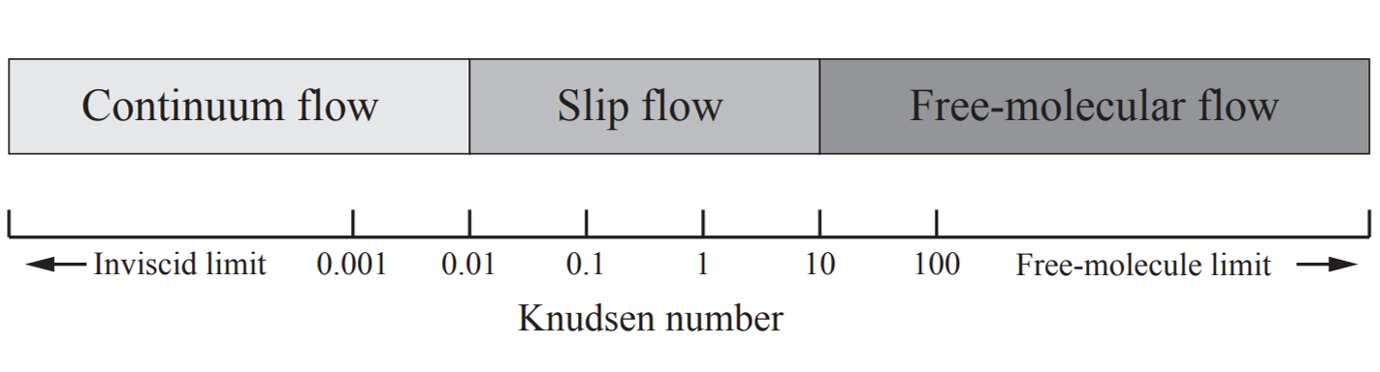
\includegraphics[width=0.7\textwidth]{../Images/2. Background/regimes.png}
    \caption{Flow regime with varying Knudsen number \cite{aerothermonotes}.}
    \label{fig:regimes}
\end{figure}

\begin{figure}[ht]
    \centering
    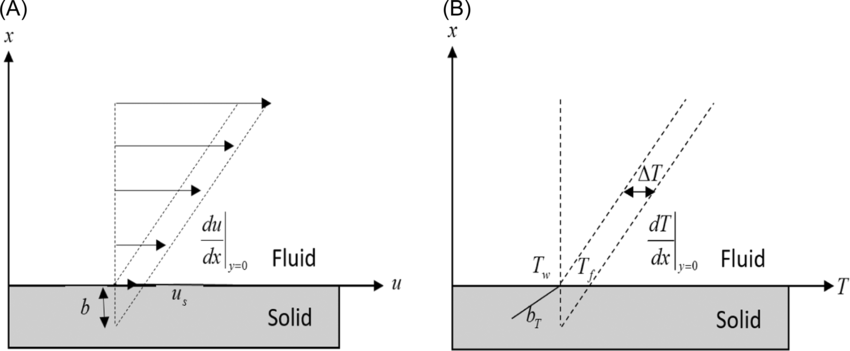
\includegraphics[width=0.7\textwidth]{../Images/2. Background/slipjump.png}
    \caption{Schematic diagram of velocity slip (A) and temperature jump (B)  \cite{slipjump}.}
    \label{fig:slipjump}
\end{figure}
It is important to note that while a flow may be globally continuous, certain local regions may exhibit signs of rarefied flow. An illustrative example of this phenomenon is the re-entry path of the space shuttle. While at a certain altitude the global Knudsen number, calculated based on the length of the vehicle, may fall within the continuum regime, the Knudsen number associated with the flow around one of the rivets on its wing could differ significantly, potentially resulting in a different regime altogether.

Precisely this intriguing dichotomy served as the explicit catalyst for this research project: as previously mentioned, the HATHOR aeroshell was analysed through both an experiment and CHT CFD \cite{hathoraero2}. This analysis was conducted on four different geometries: sharp (shown in \autoref{subfig:a}, which represents the frontal shape of HATHOR), shoulder (shown in \autoref{subfig:b}, which has an open backshell to investigate the effect of the low thickness of the heatshield), smooth (shown in \autoref{subfig:c}, similar to the sharp geometry but with smooth ribs to analyse the effect of ribs sharpness) and sphere cone (shown in \autoref{subfig:d}, resembling a standard, non folding aeroshell).

\begin{figure}[ht]
    \centering
    \begin{subfigure}{0.24\textwidth}
        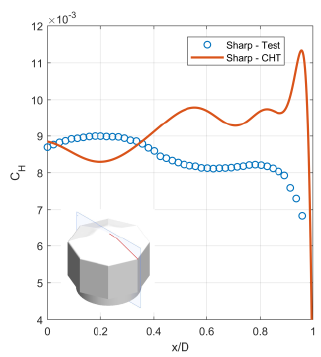
\includegraphics[width=\textwidth]{Images/2. Background/HATHOR/a.png}
        \caption{}
        \label{subfig:a}
    \end{subfigure}
    \hfill
    \begin{subfigure}{0.24\textwidth}
        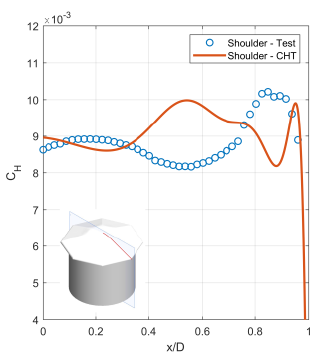
\includegraphics[width=\textwidth]{Images/2. Background/HATHOR/b.png}
        \caption{}
        \label{subfig:b}
    \end{subfigure}
    \hfill
    \begin{subfigure}{0.24\textwidth}
        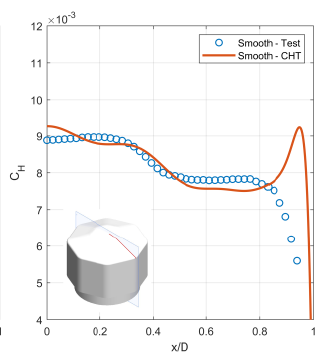
\includegraphics[width=\textwidth]{Images/2. Background/HATHOR/c.png}
        \caption{}
        \label{subfig:c}
    \end{subfigure}
    \begin{subfigure}{0.24\textwidth}
        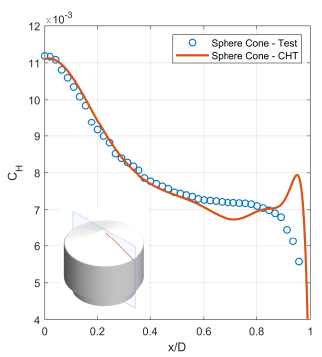
\includegraphics[width=\textwidth]{Images/2. Background/HATHOR/d.png}
        \caption{}
        \label{subfig:d}
    \end{subfigure}
    \caption{Stanton number profiles along the rib section at $\alpha=0$, $t = \qty{5}{\s}$. From the left: Sharp (a), Shoulder (b), Smooth (c), Sphere-cone (d) \cite{hathoraero2}.}
    \label{fig:hathoraero2}
\end{figure}

From \autoref{fig:hathoraero2} it is evident that significant discrepancies are present between the experimental and simulation trends. These discrepancies were the most significant in correspondence of minor geometrical features, such as the aeroshell edge and the juncture of the ribs in the sharp and shoulder models. Given the small scale of these features when compared to the geometries themselves, it was theorised that they might be inducing rarefaction effects. 

Similar patterns were noted in the analysis conducted by Rees \textit{et al.} on cubes \cite{rees}. In this paper, the hypersonic flow around cubes at incidence was analysed, both through the DLR-TAU CFD code and through a wind tunnel experiment. \autoref{fig:rees} highlights the significant discontinuities observed in the modified Stanton number produced by the simulation at the cube edge (corresponding to $z/L = 0$). Again, given the small dimension of the cube edge radius, it was thought they might be caused by a local rarefaction zone.

\begin{figure}[ht]
    \centering
    \begin{subfigure}{0.49\textwidth}
        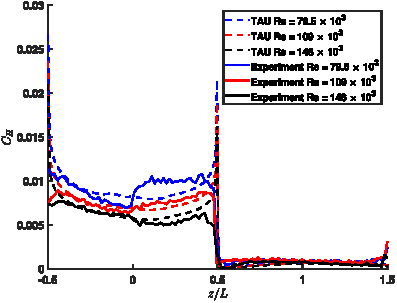
\includegraphics[width=\textwidth]{Images/2. Background/rees1.pdf}
        \caption{Windward side}
    \end{subfigure}
    \hfill
    \begin{subfigure}{0.49\textwidth}
        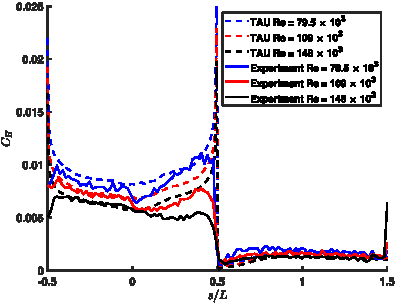
\includegraphics[width=\textwidth]{Images/2. Background/rees2.pdf}
        \caption{Leeward side}
    \end{subfigure}
    \caption{Comparisons of experimental and numerical Stanton number along the geometrical centrelines of a cube at \qty{5}{\deg} incidence, in a Mach 5 flow and at a range of Reynolds numbers \cite{rees}.}
    \label{fig:rees}
\end{figure}

To verify the aforementioned hypotheses, local Knudsen numbers were calculated for both of the experiments. Characteristic lengths of \qty{7e-4}{\m} were used for the ribs in \cite{hathoraero2} and \qty{1e-4}{\m} for the aeroshell and cube edges (taken from the machining tolerance in \cite{rees}). It was discovered that although the global Knudsen numbers were in the order of 10\textsuperscript{-5} in both the papers, local Knudsen numbers increased significantly, to the order of 10\textsuperscript{-2}, nearing the slip regime.

It was thus considered worthwhile to conduct an in depth study of the the effect of rarefaction, which is outlined in this thesis. Simple shapes were chosen for the analysis, in order to eliminate the effect that unnecessary variables, such as the half angle or the nose radius of an aeroshell, could have on the flow.

\subsection{Rarefied flow mathematical modelling}
As mentioned previously, Navier-Stokes equations cease to be valid in the rarefied flow regime. Different methods thus need to be employed for its analytical description.

Free molecular flow is modelled through the Boltzmann equation, presented in \autoref{eq:boltzmann}. This equation, developed by Ludwig Boltzmann in 1872, describes the statistical behaviour of a thermodynamic system not in a state of equilibrium. The description that it gives is in terms of microscopic quantities, such as momentum $\mathbf{p}$ and mass $m$ of the particles, and is based on a particle distribution function $f (\mathbf{x}, \mathbf{c},t)$, which expresses the probability of finding a molecule in a volume $d\mathbf{x}$ with velocity between $\mathbf{c}$ and $\mathbf{c} + d \mathbf{c}$ \cite{burnett}.
\begin{equation}
    \frac{\partial f}{\partial t}+\frac{\mathbf{p}}{m} \cdot \nabla f+\mathbf{F} \cdot \frac{\partial f}{\partial \mathbf{p}}=\left(\frac{\partial f}{\partial t}\right)_{\text {coll }}
    \label{eq:boltzmann}
\end{equation}
While this description provides an accurate representation of the system, it results to be rather complex, because of its use of microscopic quantities. Therefore, a more convenient approach would be to employ a macroscopic description of the flow, in terms of common aerodynamic quantities, such as density and flow velocity.

To solve this problem, it is possible to assume small deviations from the equilibrium conditions, and apply an expansion to the Maxwell-Boltzmann particle distribution function. This expansion is denominated the Chapman-Enskog theory \cite{burnett}, and can be seen in \autoref{eq:chapman}.
\begin{equation}
    f=f^{(0)}+f^{(1)}+f^{(2)}+\cdots=\sum_{r=0}^{\infty} f^{(r)}
    \label{eq:chapman}
\end{equation}
It is thus possible to substitute this series expansion into the Boltzmann equation, obtaining:
\begin{itemize}
    \item For a zeroth order approximation, the Euler equations of motion (accurate to order 0 in Knudsen number)
    \item For a first order approximation, the Navier-Stokes equations (accurate to order 1 in Knudsen number)
    \item For a second order approximation, the Burnett equations (accurate to order 2 in Knudsen number and shown in \autoref{eq:burnett1} and \autoref{eq:burnett2})
    \item For a third order approximation, the Super Burnett equations (accurate to order 3 in Knudsen number)
\end{itemize}
\begin{equation}
    \begin{aligned}
        P_{i j}^{(2)}=\omega_1 \frac{\mu^2}{p} \frac{\partial u_k}{\partial x_k} S_{i j}+\omega_2 \frac{\mu^2}{p}\left\{\frac{\partial}{\partial x_{\langle i}}\left(F_{j\rangle}-\frac{1}{\rho} \frac{\partial p}{\partial x_{j\rangle}}\right)-\frac{\partial u_k}{\partial x_{\langle i}} \frac{\partial u_{j\rangle}}{\partial x_k}\right.  \left.-2 \frac{\partial u_k}{\partial x_{\langle i}} S_{j\rangle k}\right\} \\
        \quad + \omega_3 \frac{\mu^2}{\rho T} \frac{\partial^2 T}{\partial x_{\langle i} \partial x_{j\rangle}}+\omega_4 \frac{\mu^2}{p \rho T} \frac{\partial T}{\partial x_{\langle i}} \frac{\partial p}{\partial x_{j\rangle}}+\omega_5 \frac{\mu^2}{\rho T^2} \frac{\partial T}{\partial x_{\langle i}} \frac{\partial T}{\partial x_{j\rangle}} +\omega_6 \frac{\mu^2}{p} S_{k\langle i} S_{j\rangle k}
    \end{aligned}
    \label{eq:burnett1}
\end{equation}

\begin{equation}
    \begin{aligned}
        q_i^{(2)}  =\theta_1 \frac{\mu^2}{\rho T} \frac{\partial u_k}{\partial x_k} \frac{\partial T}{\partial x_i}+\theta_2 \frac{\mu^2}{\rho T}\left\{-\frac{2}{3} \frac{\partial}{\partial x_i}\left(T \frac{\partial u_k}{\partial x_k}\right)-2 \frac{\partial u_k}{\partial x_i} \frac{\partial T}{\partial x_k}\right\} \\
         +  \theta_3 \frac{\mu^2}{\rho p} S_{i k} \frac{\partial p}{\partial x_k}+\theta_4 \frac{\mu^2}{\rho} \frac{\partial S_{i k}}{\partial x_k}+3 \theta_5 \frac{\mu^2}{\rho T} S_{i k} \frac{\partial T}{\partial x_k}
    \end{aligned}
    \label{eq:burnett2}
\end{equation}

More details about the derivations can be seen in the flowchart in \autoref{fig:flowchart} and in \cite{burnett}.

\begin{figure}[ht]
    \centering
    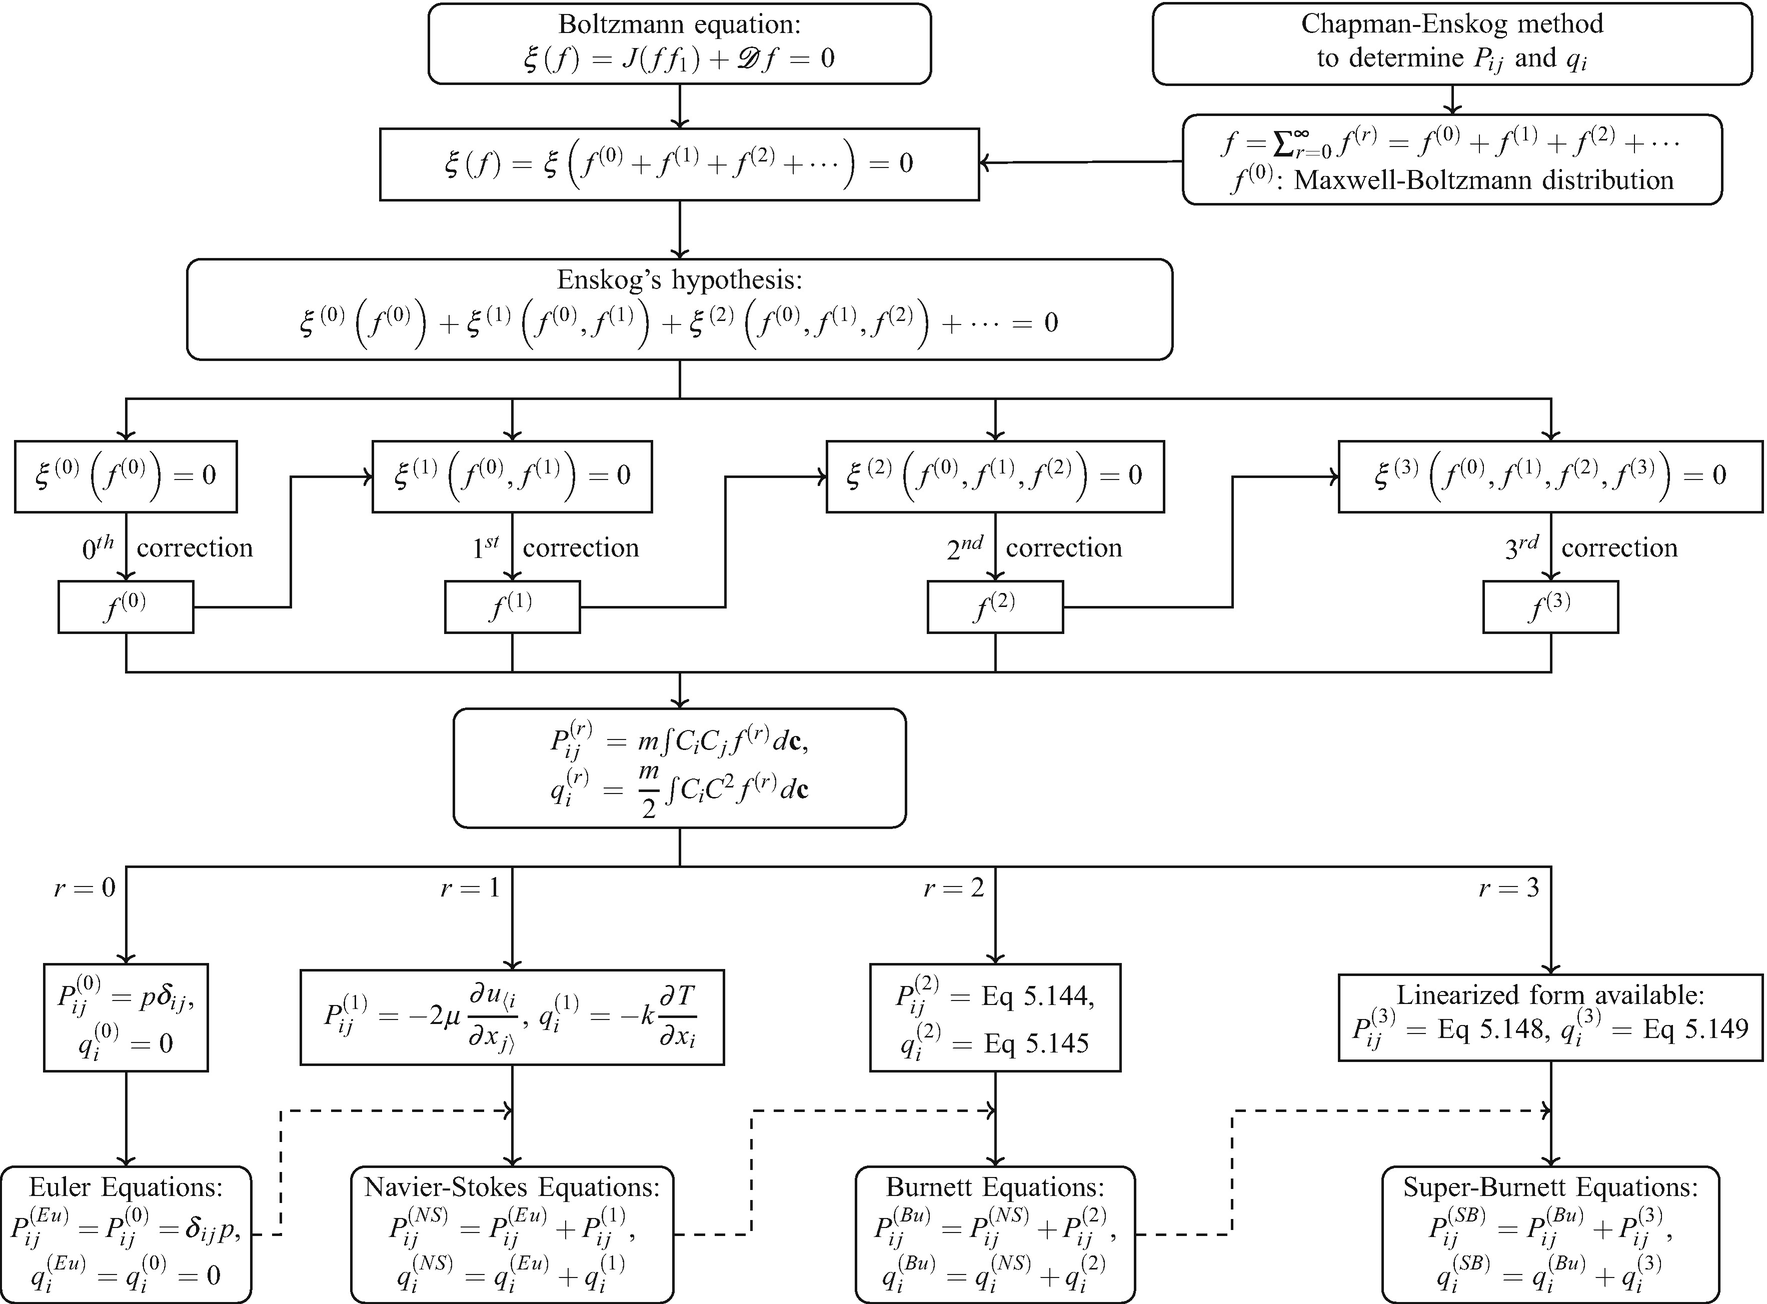
\includegraphics[width=0.9\textwidth]{../Images/2. Background/burnettflowchart.png}
    \caption{Flowchart of Burnett and Super Burnett equations derivation \cite{burnett}.}
    \label{fig:flowchart}
\end{figure}

It has been noted by the author of this dissertation that these equations, despite providing a correct analytical description of rarefied flows, are seldom to never used in literature for carrying out actual flow simulations. This is probably due to the existence of analytically simpler methods (which will be discussed in the following section), the difficulty of correctly computing accurate boundary conditions for Burnett equations and their linear instability to short wave disturbances \cite{comprarefied}.

\subsection{Rarefied flow simulation techniques}
Rarefied flow simulations are mainly divided into two categories: regular CFD codes with correction factors, and Direct Simulation Monte Carlo (DSMC) solvers.

\subsubsection{Correction model studies}

Correction models focus on modifying regular CFD codes with thermal conduction (mostly based on the Navier-Stokes-Fourier equations) to account for velocity slip and temperature jump. They are used for very diverse conditions, from rarefied hypersonics to micro scale flows for Micro-ElectroMechanical Systems (MEMS). A sample of these studies is presented below.

De Giorgi \textit{et al.} \cite{unisalento} analysed the supersonic rarefied flow onto a planar micro-nozzle through 2D and 3D CFD simulations with a maxwellian slip condition. Le \textit{et al.} \cite{le} employed the same correction factor with second order accuracy, for the study of the flow around a 25-\qty{55}{\deg} degree biconic and a NACA 0012 aerofoil. An improvement in results was noticed for the aerofoil, but performance remained unchanged for the biconic. Bhagat \textit{et al.} applied a Knudsen layer correction factor to both micro scale flows (on a backwards facing step geometry) \cite{bhagatmicro} and full-scale hypersonic flows (on a flat plate and a cylinder geometry) \cite{bhagatmacro} noticing significant improvements in both when compared to the uncorrected CFD simulations.

Nevertheless, all of these studies reveal that the performance of correction factors falls short when compared to Direct Simulation Monte Carlo, which consistently serves as the benchmark for these techniques. Based on this evidence, it was decided to employ Direct Simulation Monte Carlo for this study.

\subsubsection{DSMC studies}

Quite extensive literature exists regarding DSMC studies of various geometries. 

A significant number of studies are centered around cavities: Guo \textit{et al.} \cite{guo} investigated the effect of the length to depth ratio of the cavity in the continuum, slip and transition flow regimes, characterising the flowfield inside the cavity based on these parameters. The effect of varying Knudsen number was investigated by Nabapure \textit{et al.} \cite{nabapurecav}, who observed significant variations in the Stanton number profiles at the base and on the surfaces upstream and downstream of the cavity. Jin \textit{et al.} investigated the effect of cavity corner rounding \cite{jinrounding}, identifying a significant reduction in heat transfer to the cavity floor with the increase in radius of the aft corner.

Forward and backwards facing steps have been also analysed in depth. Nabapure \textit{et al.} investigated the effect of mach number and wall temperature on a backwards facing step \cite{nabapuremach}, and of mach number \cite{nabapuremachfor}, expansion ratio \cite{nabapureexp} and Knudsen number \cite{nabapurekn} on a forward facing step. The most relevant findings were the relative independence of wall temperature on the aerodynamic properties when compared to mach number, the variation in velocity profiles and heat transfer magnitudes on the forward facing step with Knudsen number, and the flow behaviour becoming independent of expansion ratio as expansion ratio itself was increased.

Blunt bodies, such as aeroshells or cylinders, are often chosen as the benchmark for validating DSMC codes or novel concepts in the statistical simulations domain. Palharini \textit{et al.} \cite{pallahrini} validated the dsmcFoam solver on Hypersonic rarefied non-reacting gas flows using the Mars pathfinder aeroshell geometry, noting good agreement with experimental evidence. The SPARTA DSMC code was validated on the same geometry, and on a 25-\qty{55}{\deg} biconic \cite{spartavalid}, again finding good agreement with experimental evidence. Both of the papers noted an increase in heating at the aeroshell edge with an increase in angle of attack. Malaikannan \textit{et al.} \cite{malaikannan} validated an hybrid DSMC-dynamic collision limiter code on a blunt body and aerospike geometry, discovering significant reduction in computational time and negligible differences in results when compared to the standalone DSMC code. Zhonghua \textit{et al.} \cite{zhonghua} coupled instead a regular CFD code with DSMC, assigning domain regions to each based on the local Knudsen number. Again, good agreement was found with conventional DSMC codes.







